\documentclass{article}
\usepackage{spconf,amsmath,epsfig}
\usepackage[caption=false]{subfig}
\usepackage{epstopdf}

\newenvironment{packed_enum}{
\begin{itemize}
  \setlength{\itemsep}{1pt}
  \setlength{\parskip}{0pt}
  \setlength{\parsep}{0pt}
}{\end{itemize}}

\pagestyle{empty}
\begin{document}\sloppy
\topmargin=0mm			


\title{
Selective Removal of Extraneous Photographs
}

\name{K. Armin Samii, Allison Carlisle, Uliana Popov, James Davis}
\address{[ksamii,acarlisl]@ucsc.edu,[uliana,davis]@soe.ucsc.edu}

\maketitle	
\begin{abstract}
In this paper, we propose a method for selecting the most representative high-quality images from a set of user photographs. To avoid redundancy arising from many similar images, we find all sets of near-duplicates. We then rank images based on three technical qualities: exposure, blur, and color harmony. Finally, we provide an ordering of the images which accounts for both quality and uniqueness. Our goal is not to rank images based on subjective aesthetic qualities, but instead to help a photographer filter out technically flawed photographs and focus on objectively high quality shots.
\end{abstract}	

\begin{keywords}
image processing, quality screening, exposure, meta data, color content  %image colour analysis , image segmentation , meta data , camera blur , digital albuming , quality screening , exposure , color content
\end{keywords}

\section{Introduction}
\label{sec:intro}
%With the ease of digital cameras, both amateur and professional photographers take more pictures than they will need. An organized user will delete excess photos and keep the most important ones. We need something like: The digitalization has led to an ever increasing size of personal photo collections. Today, consumers often take hundreds or even thousands of pictures of an event.

The ease of using digital cameras allows for a large number of photographs to be taken at any given event. This increase in photograph quantity can lead to many unneeded low-quality photographs that need to be filtered by the user, which can be time-consuming and repetitive.

To automate this process, an aesthetics ranking technique could be implemented to find the appeal each image has, but this method would discard many images with potential to be fixed through retouching.

%So, a technical quality ranking technique can implemented, and the best images would be kept and the worst discarded. This method solves the previous problem, but does not take into account the redundancy of similar images, and the user would be left with a set which does not span their entire photo set.

Implementing a technical quality ranking technique will keep the photographs suited for retouching, but does not take into account redundancy of similar images, and the user would be left with a set which does not span the entire event.

%To fix this, a similar image detector could be implemented giving the user the best image from every subset of similar images. This is still not ideal because it would leave the user with too many low-quality photographs that, although unique in the set, are not worth keeping.

We thus propose a technique which ranks images based on their technical qualities with a bias for unique images.%, but without forcing uniqueness by selecting the best from each set.

To focus our research and determine which image qualities are relevant to technical image quality, we assume three general steps a photographer takes between shooting and using a picture, which we call the Photographer's Process:
\begin{enumerate}
\item Remove: Sort through the imported images and remove the ones least suited for retouching.
\item Retouch: Modify the raw files just selected to stylize and enhance them.
\item Retrieve: Select the retouched images most suitable to a given task.
\end{enumerate}

We implement three modules to assess technical quality. The blur detection looks at the gradient magnitude of edges and the similarity to a predicted out-of-focus image. Exposure is measured by finding the balance in brightness throghout the image. Color harmony is based on Cohen's model\cite{Cohen-Or:2006:CH:1179352.1141933}. Similar-images are clustered into groups using the color content and timestamps of an image. Finally, a reordering of the set is provided based on how suited they are for removal (the "Importance Order"). A user study has shown 86\% accuracy in our absolute ranking of photographs and 78\% accuracy in determining which photographs belong to the same set. % 86% comes from our average difference to turk ratings on Ke's set = 1.35

\section{Related Work}

Previous works have classified images based on a professional vs. amatur photographer binary with high accuracy\cite{1640788}\cite{springerlink:10.1007/11744078_23}\cite{springerlink:10.1007/978-3-540-88690-7_29}, which is useful for search engines' retrieval of high quality images. Others have focused on personalized aesthetic rankings of photographs\cite {Sun:2009:PAB:1631272.1631351}\cite {Yeh:2010:PPR:1873951.1873963}. These works focus on finalized images, while we focus on images that are still raw and may be retouched afterward.

Event classification has been explored in order to choose the best images from an entire event\cite{1223566}\cite{4444209}, while we choose the best images from each scene within each event: images with the same subject content rather than the same event context.

Kormann, Dunker, and Paduschek\cite{springerlink:10.1007/978-3-642-10543-2_23} describe a promising method of automatically rating and ranking images based on image content and time-metadata, with results better than random. We improve upon their work with more accurate algorithms.

%Various publications have focused on improving the quality of an image, which is the second step of the Photographer's Process\cite{Bhattacahrya:2010:FPA:1873951.1873990}\cite{Kopf:2008:DPM:1409060.1409069}. 

%Others deeply researched assessing quality for the purposes of photograph retrieval from a web or multi-contributor set \cite{Yeh:2010:PPR:1873951.1873963}\cite{vanZwol:2010:FEI:1772690.1772788}\cite{springerlink:10.1007/978-3-642-17187-1_57}\cite{Cui:2008:RTG:1459359.1459471}\cite{Chu2010256}. 

%Previous works in image quality assessment have ranked image quality based on relevancy and quality 
%%blur \cite{springerlink:10.1007/978-3-540-77409-9_26}, exposure \cite{5540170}, color harmony \cite{COL:COL5080160410}\cite{COL:COL10004}, and duplicate detection \cite{Chu2010256}. %User tags on Flickr and online search engines have provided sets of similar images to compare\cite{Berg:EECS-2007-13}\cite{Chu2010256}. 
% Duplicate detection isn't quality assessment though?

%%Several papers have developed methods for separating professional and amateur photographs \cite{springerlink:10.1007/978-3-540-30541-5_25}\cite{springerlink:10.1007/11744078_23}\cite{1640788}\cite{springerlink:10.1007/978-3-540-88690-7_29}. %Unlike our work, these assume a finalized image. 

%The methods for image retrieval are not as useful for image removal because they assume a finalized photograph, rather than looking at the potential to be enhanced- or, more simply, they focus on aesthetic quality over technical quality. Removal of technically flawed photographs, as opposed to aesthetically unpleasing ones, is more readily automated without consideration of personal preference. We consider color harmony a technical aspect because it can be indicative of probems with lighting and color balance.

%%Compressed image quality assessment has been heavily researched\cite{477498}\cite{1038064}\cite{1284395}, but we assume a high quality import. As described in \cite{1315222}, a photograph's EXIF data can be used to robustly classify images into various semantic categories. Various aesthetic-based assessments focus on exploring human visual attention and sensitivity to photograph content\cite{Sun:2009:PAB:1631272.1631351}\cite{1518955}\cite{Pimenov_fastimage}, demonstrating the viability of content segmentation for image assessment.

\section{Quantifying Image Quality}
\begin{figure*}
  \centering
    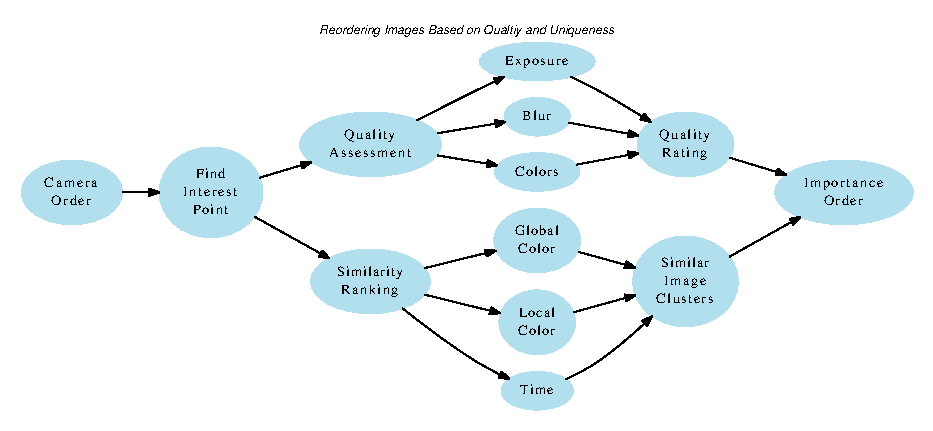
\epsfig{file=flowchart.eps,width=16cm}
  \caption{Interest points are used to find the subject. Blur detection, color harmony, and exposure algorithms calculate an image's quality rating. The color distribution of the local subject and global image, coupled with the timestamp, cluster images into groups. A reordering of the input results, allowing the user to remove images at the end of this ordering.}
  \label{flowchart}
\end{figure*}

To find the Importance Order of the user's photographs, we first use interest points to find the subject, which will be used for both quality assessment and similarity clustering. Quality is determined by the rankings of the blur, exposure, and color harmony modules. Groups of similar images match the color content and timestamp of every pair of images. We combine them to get the final ordering (Fig. \ref{flowchart}).

The blur, exposure, and color assessment modules will provide a ranking between zero and nine, with larger numbers indicating higher quality. Because an image which is flawed in any of the three factors would be considered poor, we propose a formula which penalizes low scores more than it rewards high scores:
\begin{eqnarray}
\left(\displaystyle\sum\limits_{i=1}^nW_i\left({Q_i+t}\right)^\frac{2}{3}\right)^\frac{3}{2}
\end{eqnarray}
Where:
\begin{packed_enum}
\item \textbf{\(n\)}: Number of modules
\item \textbf{\(W_i\)}: Weight of module \(i\)
\item \textbf{\(Q_i\)}: Rating produced by module \(i\)
\item \textbf{\(t\)}: A leniency threshold to balance each module's output
\end{packed_enum}
And weights assigned as follows:
\begin{packed_enum}
\item \(W_{exposure}=30\%\)
\item \(W_{blur}=60\%\)
\item \(W_{color}=10\%\)
\end{packed_enum}

\subsection{Subject Recognition}\label{ContentRecognition}
Using a Harris Interest Operator (utilizing NASA's Vision Workbench\cite{vision-workbench}) interest points are obtained for each image. To extract a bounding box from these points, the most dense rectangle is calculated by maximizing the ratio of interest points to rectangle area. We assume this to be the primary subject. It is used in detecting similar images and calculating blur levels. 
%Although there are more accurate methods available\cite{5649226}, our work only requires this simpler method which provides a bounding box around the most salient foreground object.

\subsection{Similar-Image Clustering}
To find similar images we perform three steps of increasing complexity for high confidence.
%\begin{figure}
%  \centering
%    \epsfig[scale=0.07,clip]{similarimages.eps}
%  \caption{We cluster images based on their temporal nearness, overall color distribution, and foreground subject color distribution.}
%\end{figure}
First, we use the timestamp to obtain a similarity index between all pairs of images. Based on a formula which groups photos by finding large timestamp gaps\cite{1292402}, we have derived a formula which finds temporal closeness between every pair of images. So, instead of finding gaps in sets, we find the similarity \(S_{i,j}\) between two images \(i\) and \(j\) on a 0-9 scale. This allows nonconsecutive images to be grouped together:
\begin{eqnarray}
S_{i,j}=\frac{G_{i,j}}{A_{i,j}}
\end{eqnarray}
Where \(A_{i,j}\) is the average gap within a window size of 8 images before \(i\) and after \(j\), and  \(G_{i,j}\) is the log of the time gap between the two images taken at time \(T_i\) and \(T_j\):
\begin{eqnarray}
G_{i,j}=\log(|T_i-T_j|)
\end{eqnarray}
The calculated similarity index \(S_{i,j}\) is used to weight the results of the next two steps.

The image is then divided into a 4x4 grid of average color values. To compare two images, we find the color difference of each square (average difference of the red, green, and blue channels) and deduct from the similarity score if the difference is greater than a threshold of 15\%. Because this is sensitive to subject and camera movement, we then take the bounding box derived in \ref{ContentRecognition} and rerun the difference algorithm with stricter threshold of 10\%.

Clusters are formed using a Quality-Threshold algorithm. We first put each image into its own group, then iteratively merge the two most similar groups until a minimum similarity threshold is reached. In this way, groups votes for other similar groups, rather than single image voting for other images, resulting in a noise-resistant clustering. This method successfully groups panoramic sets of images together, even when the first image's color does not match the last image's. % Add panorama image?

\subsection{Blur Detection}
Using the foreground bounding box, the blur detection algorithm first quantifies the spread of the subject's edges. Using the Image Gradient Model proposed in \cite{springerlink:10.1007/978-3-540-77409-9_26}, we obtain a value for the blur.

Next, we compute a predicted blurred model of the foreground using a gaussian function. Sharpness is determined by an image's similarity to the predicted blur model, with sharp images being the least similar. These two values combine to determine the amount of blur, which is especially accurate when comparing the foregrounds of two similar images.

\subsection{Exposure}
\begin{figure}
  \centering
    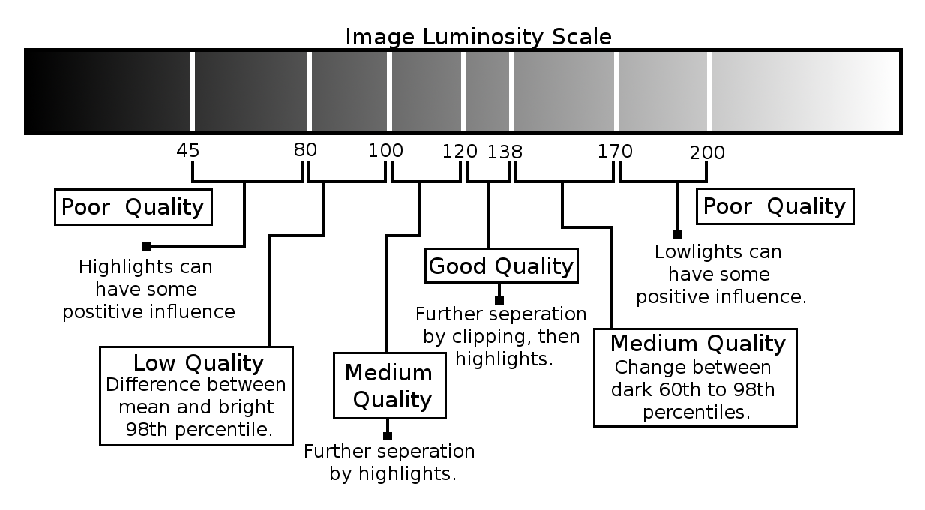
\epsfig{file=imageluminosity.eps,width=8.5cm}
    \caption{The exposure process: This figure shows the inital segmentation of images by mean luminosity, then the further segmentation of images of medium and high quality (mean ranges 100-120 and 120-138 respectively).}
    \label{exposurefigure}
\end{figure}
Image exposure is a measure of how appropriate the lighting is in a given image. While easily measured in-camera using a light meter, we must evaluate the lighting condition based on pixel intensity. Images are ranked according to various measures of their brightness. %The calculation for brightness used is
%\[
%p=.59r+.3g+.11b
%\]
%where \(p\) is the perceived intensity, and \(r\), \(g\), and \(b\) are the red, green, and blue components, respectively(XX THIS FORMULA NEEDS REFERENCE).

We have determined eight measures by examining a set of images with various exposure problems. The measures relevant to exposure quality are: clipping, highlights, lowlights, the upper 60th and 98th percentiles, the lower 60th and 98th percentiles, and variance. Each of these measures is calculated on both the subject and the background of the image, relative to the area over which it is calculated.

Based on the idea that the mean value of image brightness is an approximate indication of how well-exposed an image is, images are first segmented based on their mean brightness value ("mean"). The categories for the mean correspond roughly to a parabolic mapping of exposure values (Fig. \ref{exposurefigure}), with well exposed photographs having a mean value between 130 and 140. The further towards the extreme high and low means, the worse quality the image is. These divisions are used as the starting point of analysis. %Within each category, different measures indicate either a positive or negative overall impact on image quality, which impact depends upon the various categories. For example, in an overall dark mean, having more extreme bright areas makes the image more balanced, while in a bright image they usually indicate that it has been overexposed.

%Overexposure of an image can lead to large areas in the photo in which the human eye cannot discern any form (note that this definition can also indicate areas of a solid white value that contains absolutely no data about the form present). However, as the program is primarily concerned about how humans perceive images, the number of pixels in the highest five perceived values are used to calculate the “highlights” present in the image.

%Lowlights can be caused by underexposure, but they can also be a product of poor lighting (e.g., photographing a shadowed object in extremely bright conditions). Again, some lowlights are desirable for contrast in an image, but too much leads to an undecipherable image.

%Clipping is an indication of how much information loss there is in the image. %due to extreme shadows and bright spots, measured as a sum of the Highlights and Lowlights.

%The percentiles of the image are determined for both the bright and the dark sides of brightness. For example, to calculate the lower 60th percentile, the value is found at which the sum of the number of pixels that are darker than the given value is equal to sixty percent of the pixels in the image. The upper percentiles are found by the summation of the pixels that are brighter than the given value. These four measures give a good indication of the spread of the brightness, e.g., how sharp the transitions between the extreme and middle values are.

The most extreme mean brightness values are images of very poor quality, and are rated as such based solely on the mean value. Means between 80 and 170 encompass nearly all images of acceptable to excellent exposure, and thus require the most the analysis. After being subdivided into mean categories, they are again subdivided into further categories before analysis.

We use the mean value, categories, subcategories, and the eight measures to determine if the exposure is balanced throughout the image. An image with a dark mean should have bright pixels, and an image with a light mean should have dark pixels. An unbalanced image is rated poorly, even if it has an acceptable mean. Well-balanced images within the acceptable mean range are rated highly.

\subsection{Color Harmony}   
%\begin{figure}
%  \centering
%    \epsfig[scale=0.38,clip]{colorharmony.eps}
%  \caption{The harmonies described in \cite{COL:COL10004} are used to find the quality of the relationships between colors.}
%\end{figure}

To determine the quality of a photograph's color content, we use Cohen's seven types of color harmony\cite{Cohen-Or:2006:CH:1179352.1141933} to determine which, if any, is contained in the photograph. For each image, we find the hue which is most represented across the seven types, as well as the percent of pixels which match any of the harmonies.

We separate the pixels into bins based on their saturation values, using user-study data from Amazon Mechanical Turk to determine the boundaries of each bin. We then look for the most closely matched harmony type within each bin, ranking the bin based on how far it is from the closest type. We combine the bins' rankings for a final quality ranking.

%The first harmony checked is the average and great image's I type. If there is a large amount of I harmony, the difference between I and Y harmonies is checked. Because I and Y overlap, you need to check how much of an increase if between the two. If it is very significant, Y harmony is most likely. When the difference is slight, you have a good I harmony (and thus high rating). If there is a medium difference, the I harmony is weak. Rating of the images can be determined on medium to great harmony. A similar check is done in X versus Y harmony. A last pass is done to check the L type on the great images, and a pass checking the v and i harmonies is done on the average images.

%The poor images follow a similar path, starting with analysis by the X harmony, and ending with a pass done with i harmony.

\section{Results}
We have run our algorithm on several publicly available datasets as well as our own. We used Amazon Mechanical Turk and gathered a total of 454 users rankings across trials.

Enumerated below are the results and comparisons to similar works.

\subsection{Similar Image Detection}
We asked Turk users to group together photographs within four sets of twenty images based on their own personal measure of "similarity." Our similarity ranking module agreed with Turk users with 78\% accuracy. We then grouped together photographs with the same subject in focus and achieved an 85\% accuracy on the same dataset. % JAMES SHOULD THIS LAST MEASURE BE HERE?

\subsection{Image Rating}
\begin{figure*}[t]
\centering
\subfloat[
Blur: 2.4 \(\mid\)
Exposure: 6 \(\mid\)
Color: 4]
{
	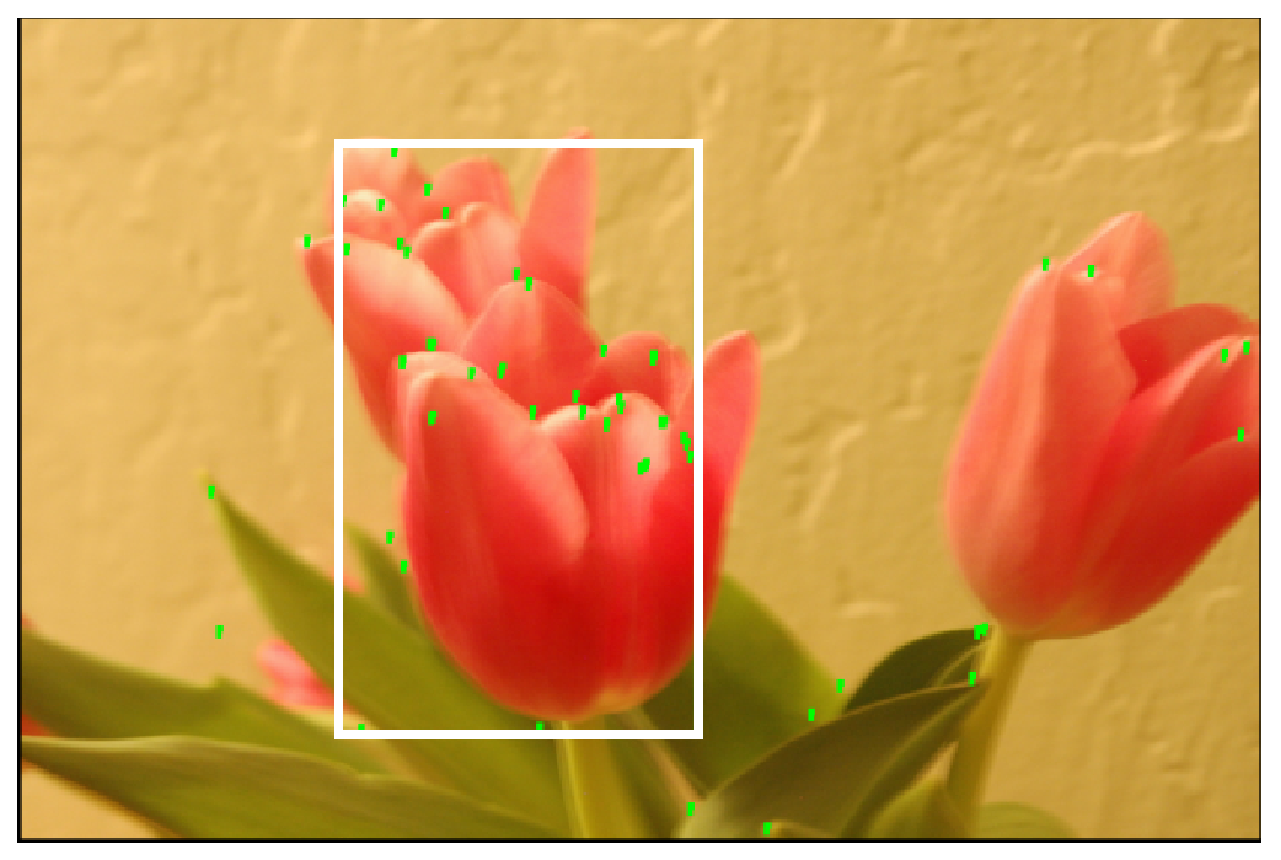
\epsfig{file=example_blur.eps,width=5cm}
	\label{example_blur}
}
\subfloat[Blur: 6 \(\mid\)
Exposure: 1.2 \(\mid\)
Color: 1]{
	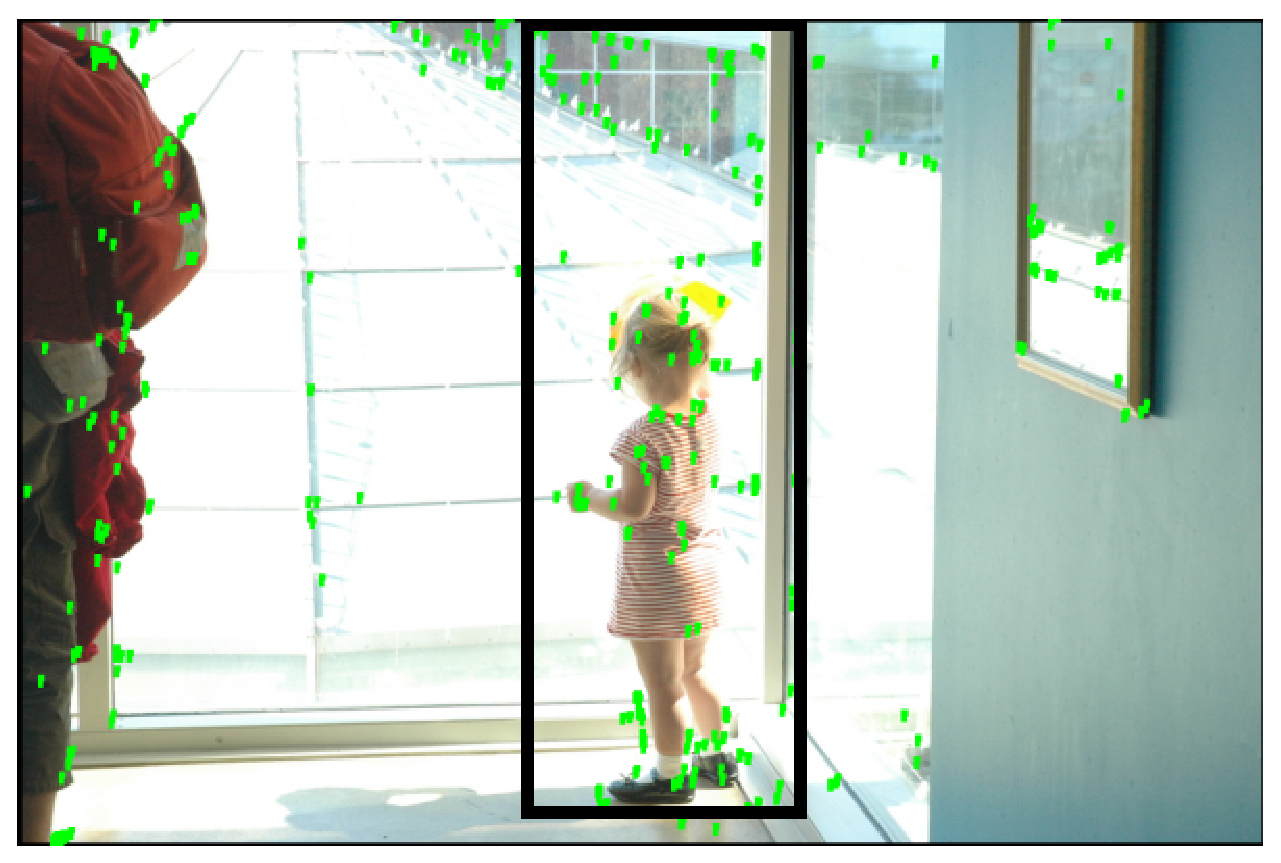
\epsfig{file=example_expose.eps,width=5cm}
	\label{example_expose}
}
\subfloat[
Blur: 9 \(\mid\)
Exposure: 7.4 \(\mid\)
Color: 7]{
	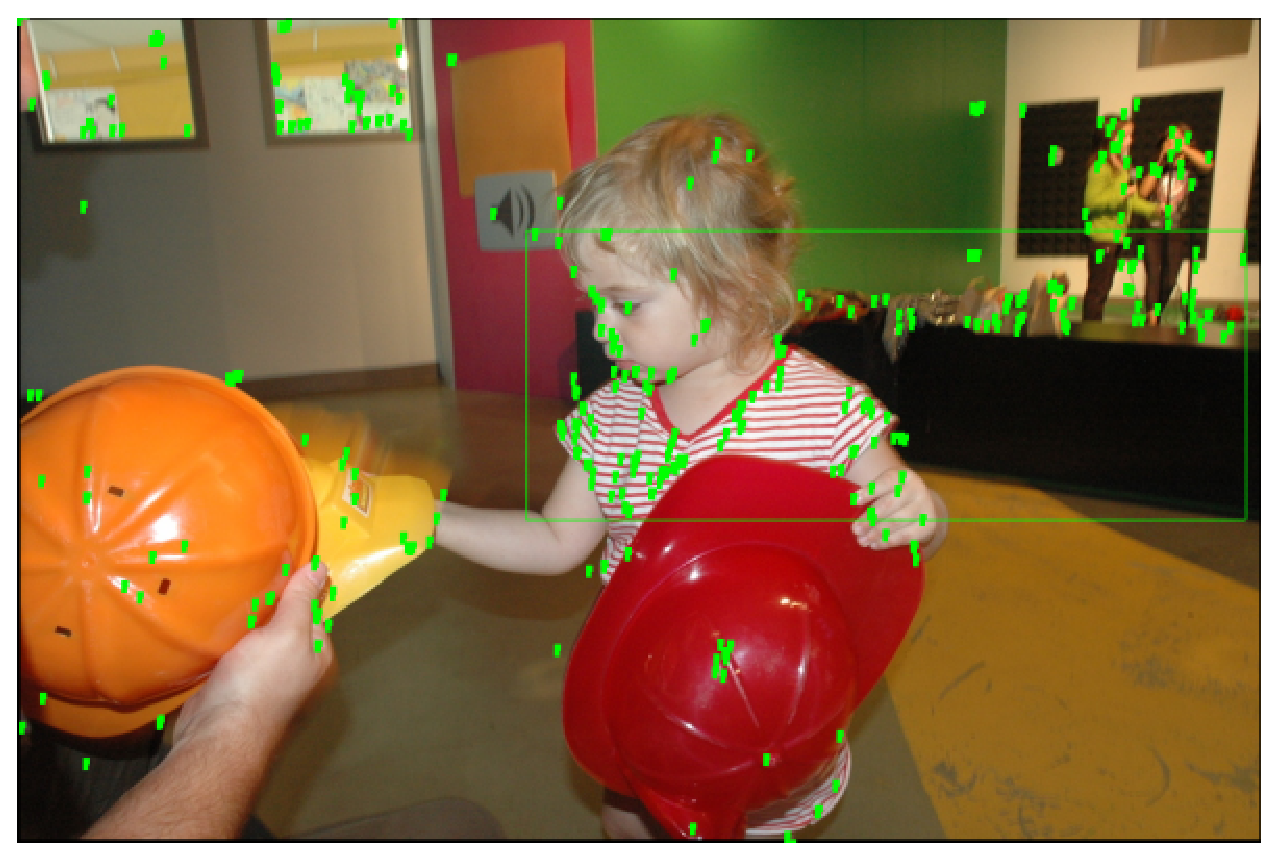
\epsfig{file=example_good.eps,width=5cm}
	\label{example_good}
}
\caption{Examples of \subref{example_blur}\subref{example_expose} low quality and \subref{example_good} high-quality images. The dots are interest points found; the square is the bounding box considered to be the subject. Despite the too-inclusive box in \subref{example_good}, each algorithm worked properly.}
\label{fig:Examples}
\end{figure*}

Separate trials were run to compare our algorithm to previously ranked images: 48 from Ke, Tang, and Jing\cite{1640788}, and 100 from Luo and Tang\cite{springerlink:10.1007/978-3-540-88690-7_29}. We then compared 459 of our own images to Turk users. Here we compare against an absolute rating of each image without regard to the sets of similar images.

Using the 48 image data set from Ke, Tang, and Jing\cite{1640788}, and Amazon Turk ratings as a ground truth, we achieve a correlation coefficient of \(.340\), which is comparable to the authors' correlation coefficient of \(.495\). Similarly, with a random sample of 100 images from Luo and Tang's public data set of high-quality images\cite{springerlink:10.1007/978-3-540-88690-7_29}, we achieve a correlation coefficient of \(.311\). These numbers show that our algorithm provides positive absolute results when comparing photographs independently, despite our focus on ranking images within a set of related images.

%\subsection{Binary Classification} Using the same data as the Image Rating trials, we have found that our algorithm can distinguish between professional and non-professional images well. Barsky \cite{Yeh:2010:PPR:1873951.1873963} and Luo \emph{et. al}\cite{springerlink:10.1007/978-3-540-88690-7_29} obtained 96\% accuracy when classifying images into the two categories. When classifying "non-professional" as Turk ratings below XX/9 and "professional" above XX/9, our rating system matches a user's with XX\% accuracy.

\section{Conclusion and Future Work}
We propose a method of applying current research to automate another step of the Photographer's Process. By focusing on obtaining an ordering which is representative of all photographs taken, we obtain a diverse set of high quality images similar to what a user would have chosen manually. We derive a novel algorithm for analyzing exposure quality. We improve upon previous algorithms which find temporal gaps between images to obtain a metric for temporal nearness. The final ordering depends on both the quality ranking and the number of similar images which have already appeared.

Our work focuses on a small portion of the Photographer's Process. In the future, we would like to see the idea of relative rankings applied to the second Retouching step. (It has already been extensively applied to the third Retrieval step.) Retouching can use relative processing to increase creativity between similar images or combine data from multiple images. With this, we would be able to automate the Photographic Process.

{\footnotesize
 \bibliographystyle{IEEEbib}
 \bibliography{README_BIB}
}
\end{document}
